\section{Introduction}

Automated design and synthesis of both application-specific and general-purpose
instruction-set processors is an active area of research~\cite{2006_dutt_chapter}
with instruction set architecture (ISA) design seeing new techniques and improvements~\cite{2002_qin_date}.

%Automated design of general purpose processing cores, application-specific
%instruction-set processors (ASIPs), and distributed Systems-on-Chip
%(SoCs) has gained a lot of attention from academia and industry.
%New formalisms for data-path modelling are proposed~\cite{2010_mokhov_ieee}\cite{2008_sokolov_sdfs},
%hardware/software co-design methodology~\cite{1993_alomary_edac}
%is actively developed and applied for ASIP performance improvement,
%more specific techniques (such as compiler-directed instruction set
%optimisation~\cite{2002_qin_date}) are constantly introduced into
%the instruction set architecture (ISA) design domain.

Synthesis of instruction sets is a particularly active research area.
There are methods of automated derivation of ISA for a given platform
according to available system components
and for given software requirements. These methods eventually produce a
set of instructions satisfying certain properties (orthogonality,
completeness, regularity, etc.); instructions are grouped into categories
and each category is allocated a certain opcode range within the
code space~\cite{2003_nohl_dac}. At this point automation is typically
stopped or becomes trivial: the instructions are given arbitrary codes
within the allocated ranges. This limits performance due to instruction
decoder circuitry overheads. The problem is usually approached by
ad-hoc heuristics or application-specific optimisation techniques
(see, for example,~\cite{2002_lee_iccad}).

The TPG notation has an application in CPU design with a natural hardware correspondence: it desribes synshronous or asynchronous control logic over the units defined by graph vertices. Such logic is commonly called a \emph{decoder} -- a circuit that takes an instruction code word and produces control signals for CPU components.  

In Chapter~\ref{chap:PGEncoding} we address the problem of TPG \emph{encoding}~\cite{2009_mokhov_phd} -- the process of identification of an efficient TPG from which a given set of partial orders may be obtained via the TPG specialisation mechanism. An efficient encoding makes it possible to describe systems in
a compact functional form and apply structural synthesis methods which
significantly improve performance of the whole design flow. These
features make the model very efficient for representation and management
of processor instruction sets in hardware and EDA software. 

We discuss the known TPG encoding techniques:
\begin{itemize}
\item \emph{binary encoding}, synthesising a TPG with the minimal number of variables;
\item \emph{matrix encoding}, where each vertex and arc are assigned a unique control variable;
\item \emph{one hot enconding}, attributing a variable to each unique original scenario;
\item \emph{weakly optimal encoding}\footnote{In \cite{2009_mokhov_phd}, this is referred to simply as \emph{optimal}.} finds a solution with the minimal total number of variables among the solutions with fewest literals (ground terms); like the matrix encoding, it yields a TPG with single variable conditions; however, generally, it uses fewer variables in total.    
\end{itemize}

We proceed to discuss how we improve upon this work by introducing a new algorithm. The algorithm is able to identify a globally optimal solution for a given fixed set of optimality criteria. The techniques discussed above are only able to identify various forms of local optimums. More precisely, the four existing techniques define just four points in the \emph{solution space} constructed by our algorithm. Only one of these points is located on the Pareto optimality frontier, constructed by our algorithm (see Fig.~\ref{fig:pareto}).

\begin{figure}[t]
\centering
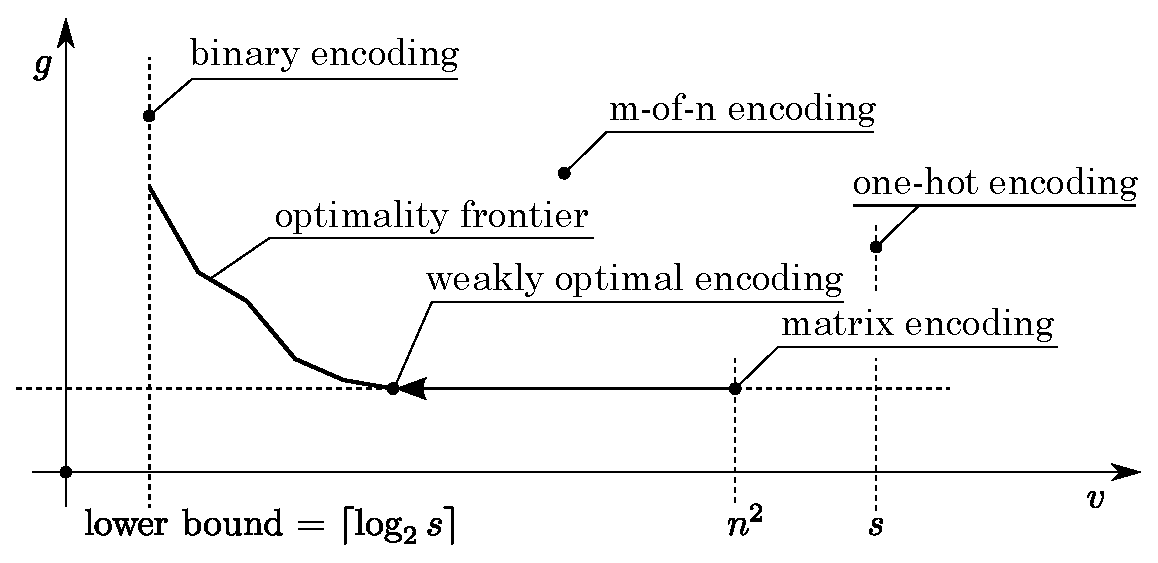
\includegraphics[scale=0.7]{fig/optimality_frontier}
\caption[The optimality frontier]{\label{fig:pareto}The relationship between the optimality frontier, as found by our algorithm, and the solutions proposed in~\cite{2009_mokhov_phd}. On the axis $g$ we plot the number of logic gates needed to describe the instruction decoder and the axis $v$ corresponds to the number of variables used to encode the instructions.}
\end{figure} 
 
The gist of the approach lies in a combination of binary search and Boolean satisfiability solving (SAT). Binary search travels through a binary tree of potential solutions using a choice function of the form $f \in D \rightarrow \mathbb{B}$ where $D$ is domain limiting the space of explored solutions. In our case, such $D$ may define either a set of gate counts of a decoder circuit or, alternatively, the set of number of variables used in TPG conditions. In a general case, $f$ takes the following form: 

$$f(x) = \left \{ \begin{array}{l} 1,~ \text{when there exists a solution} ~ S ~ \text{such that its cost is}~ x \\ 0,~ \text{otherwise}  \end{array} \right .$$   

\noindent
Such function $f$ may be challenging to compute since the set from which solutions are drawn is typically large. Let $v$ and $g$ signify the maximum number of variables and gates; also let $s$ be the number of scenarious encoded in the original TPG. Then the size of the solutions space is in the order of 

$$\left (2 (v + g) \right )^{2g} \left (2^{v} \right )^{s}$$  

\noindent For instance, for $v=5$, $g=5$ and $s=5$ the formula above gives circa $10^{21}$ potential solutions to consider. Clearly, computing $f$ with a brute-force approach is infeasible. Note, however, that $f$ has a form of an existential quantifier binding indentifiers to finite domains. This form of statement is perfectly suited for SAT solving. To bridge to the SAT-level notation we have to do binary vector encoding of scenario and variable indices, gate identifiers and cost indicators. The result is processed by a SAT solver and the output is a binary representation of a decoding circuit. In particular, we have used \noun{MiniSat}~\cite{2004_miniSAT_lncs} and \noun{clasp}~\cite{clasp} SAT solvers. As one example, we have been able to obtain an optimal solution for $v=8$, $s=8$ and $g \in 3 .. 12$.     
